%!TEX TS-program = xelatex
%!TEX encoding = UTF-8 Unicode
% Awesome CV LaTeX Template
%
% This template has been downloaded from:
% https://github.com/posquit0/Awesome-CV
%
% Author:
% Claud D. Park <posquit0.bj@gmail.com>
% http://www.posquit0.com
%
% Template license:
% CC BY-SA 4.0 (https://creativecommons.org/licenses/by-sa/4.0/)
%


%%%%%%%%%%%%%%%%%%%%%%%%%%%%%%%%%%%%%%
%     Configuration
%%%%%%%%%%%%%%%%%%%%%%%%%%%%%%%%%%%%%%
%%% Themes: Awesome-CV
\documentclass[11pt, a4paper]{awesome-cv}

%%% Override a directory location for fonts(default: 'fonts/')
\fontdir[fonts/]

%%% Configure a directory location for sections
\newcommand*{\sectiondir}{resume/}

%%% Override color
% Awesome Colors: awesome-emerald, awesome-skyblue, awesome-red, awesome-pink, awesome-orange
%                 awesome-nephritis, awesome-concrete, awesome-darknight
%% Color for highlight
% Define your custom color if you don't like awesome colors
\colorlet{awesome}{awesome-red}
%\definecolor{awesome}{HTML}{CA63A8}
%% Colors for text
%\definecolor{darktext}{HTML}{414141}
%\definecolor{text}{HTML}{414141}
%\definecolor{graytext}{HTML}{414141}
%\definecolor{lighttext}{HTML}{414141}

%%% Override a separator for social informations in header(default: ' | ')
%\headersocialsep[\quad\textbar\quad]


%%%%%%%%%%%%%%%%%%%%%%%%%%%%%%%%%%%%%%
%     3rd party packages
%%%%%%%%%%%%%%%%%%%%%%%%%%%%%%%%%%%%%%
%%% Needed to divide into several files
\usepackage{import}

%%%%%%%%%%%%%%%%%%%%%%%%%%%%%%%%%%%%%%
%     Personal Data
%%%%%%%%%%%%%%%%%%%%%%%%%%%%%%%%%%%%%%
%%% Essentials

\name{Dat-Chanh}{Nguyen}
\address{Luzernerstrasse 71, 6014 Luzern}
\mobile{(+41) 78-653-0756} 
%%% Social
\email{nguyenchanhdat@gmail.com}
%\homepage{www.posquit0.com}
\github{gipfeli}
\linkedin{gipfeli}
%\stackoverflow{1763783}{gipfeli}
%%% Optionals
%\position{Werkstudent im Bereich Gas Sensors}
%\quote{``Make the change that you want to see in the world."}


%-------------------------------------------------------------------------------
\begin{document}
\begin{minipage}{\textwidth}
% Print the header with above personal informations
\makecvheader
\end{minipage}
%\begin{minipage}{0.15\textwidth}
%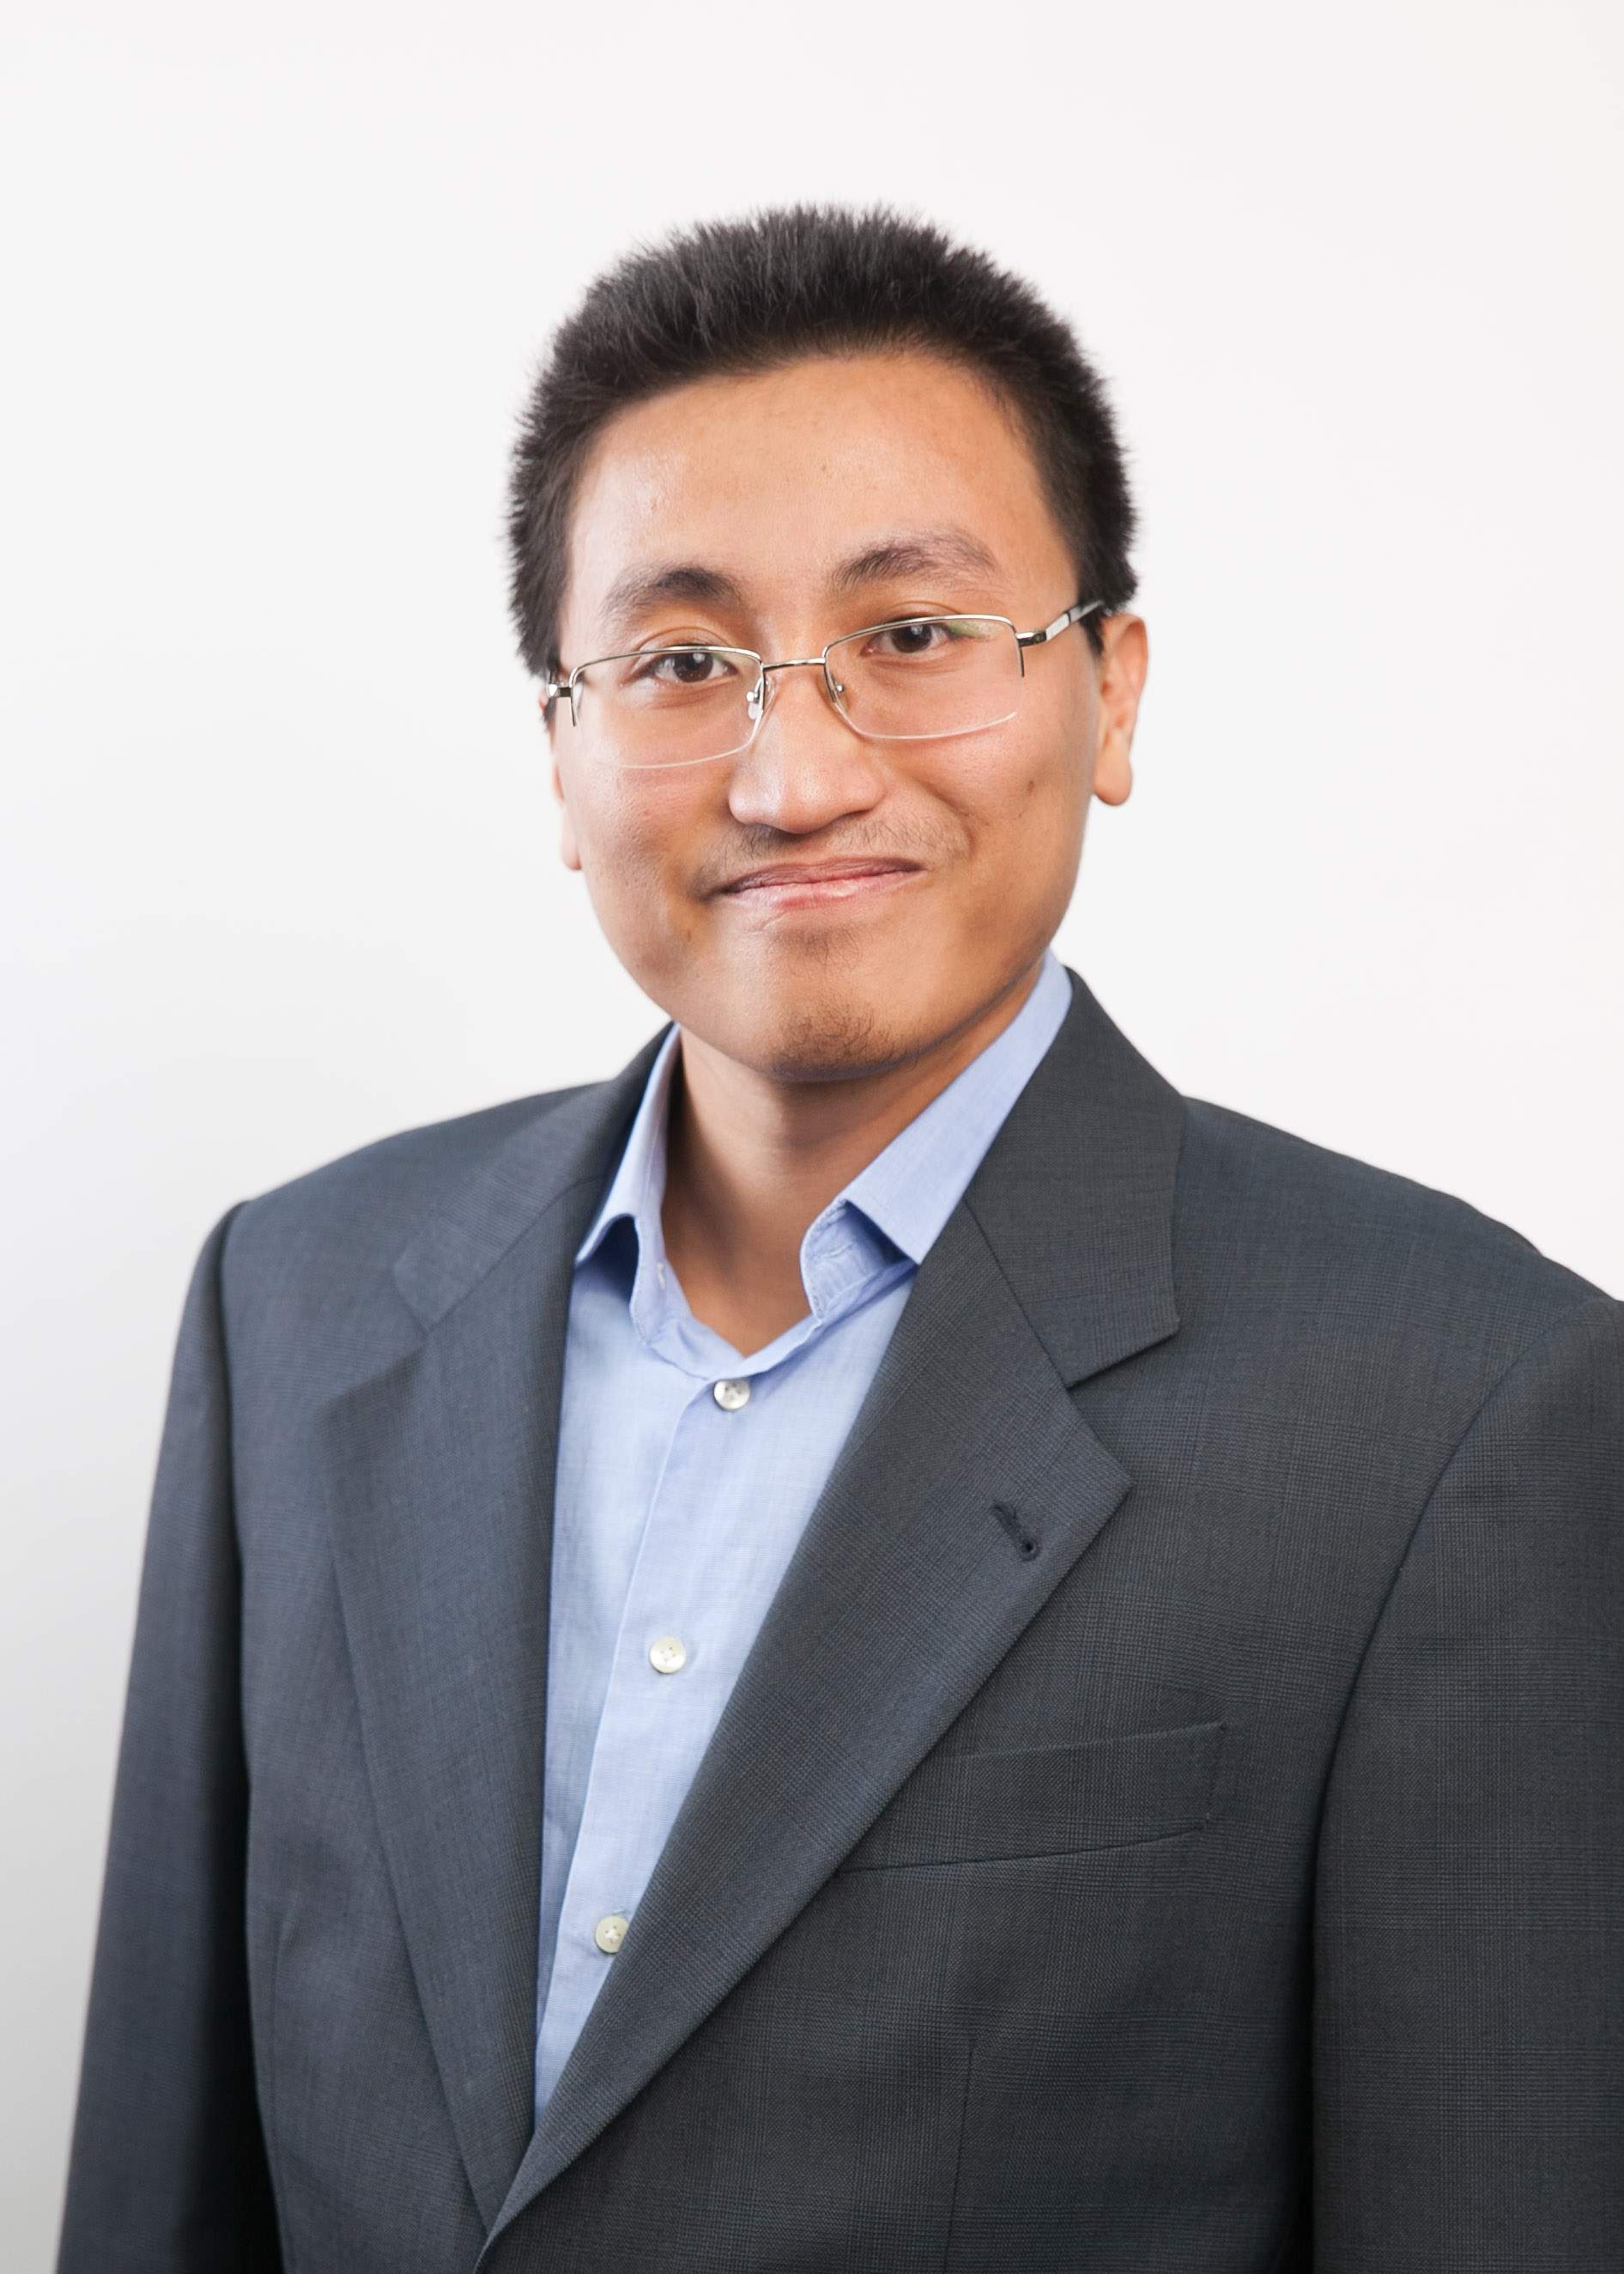
\includegraphics[width=2.75cm]{cv/photo}
%\end{minipage}

% Print the footer with 3 arguments(<left>, <center>, <right>)
% Leave any of these blank if they are not needed
\makecvfooter
  {\today}
  {Nguyen Chanh Dat~~~·~~~Curriculum Vitae}
  {\thepage}


%-------------------------------------------------------------------------------
%	CV/RESUME CONTENT
%	Each section is imported separately, open each file in turn to modify content
%-------------------------------------------------------------------------------
%-------------------------------------------------------------------------------
%	SECTION TITLE
%-------------------------------------------------------------------------------
\cvsection{Education}


%-------------------------------------------------------------------------------
%	CONTENT
%-------------------------------------------------------------------------------
\begin{cventries}

%---------------------------------------------------------
\cventry
{B.Sc. in Maschinentechnik} % Degree
{Hochschule Luzern Technik \& Architektur} % Institution
{Luzern, Schweiz} % Location
{2016 - 2020} % Date(s)
{
	\begin{cvitems} % Description(s) bullet points
		\item {\textbf{Vertiefung}: Produktentwicklung und Mechatronik}
		\item {Projekt: Realisieren ein autonomes Fahrzeug, welches einen Geländeparcours bewältigen kann}
		\item {\textbf{Abschlussthesis}: Entwickeln einen Bioreaktor als Teil des Lebenserhaltungssystem eines Space-Habitat - \newline Industrie-Partner: \mbox{SwissSpaceCenter} (SSC) \& European Space Agency (ESA - Biotesc: Biomedizinsche Forschungsgruppe) (2019)}
	\end{cvitems}
}


%---------------------------------------------------------
%  \cventry
%    {B.Sc. in Mechanienbauwissenschaft} % Degree
%    {ETH Zürich} % Institution
%    {Zürich, Schweiz} % Location
%    {} % Date(s)
%    {
%      \begin{cvitems} % Description(s) bullet points
%        \item {Teaching Assistant: Introduction to Fortran Programming}
%        \item {Programming Assistant: Data analysis with Python and PostgreSQL}
%      \end{cvitems}
%    }

%---------------------------------------------------------
%  \cventry
%    {Gymnasiale Maturität} % Degree
%    {KSR (Kantonsschule Reussbühl)} % Institution
%    {Luzern, Schweiz} % Location
%    {} % Date(s)
%    {
%      \begin{cvitems} % Description(s) bullet points
%        \item {Schwerpunktfach: Mathematik und Physik}
%      \end{cvitems}
%    }

%---------------------------------------------------------
\end{cventries}

%-------------------------------------------------------------------------------
%	SECTION TITLE
%-------------------------------------------------------------------------------
\cvsection{Skills}


%-------------------------------------------------------------------------------
%	CONTENT
%-------------------------------------------------------------------------------
\begin{cvskills}

%---------------------------------------------------------

  \cvskill
    {Engineering Tools} % Category
    {\textbf{CAD}: (UNI NX, Solidworks, Autodesk Inventor); 
    \newline \textbf{CFD}: OpenFOAM
    \newline \textbf{SPS}: TwinCAT3, Selectron CAP1131
	\newline \textbf{FEM}: Ansys (statics)\smallskip} % Skills

%%---------------------------------------------------------
%
%  \cvskill
%    {Manufacturing Tools} % Category
%    {\textbf{3D Print/CNC}: Skeinforge, G-Code;} % Skills

%---------------------------------------------------------
  \cvskill
    {Programming} % Category
    {\textbf{Languages}: Python, MatLAB; C/C++, Fortran, LaTeX 
    	\newline \textbf{Datenbank}: MySQL/PostgreSQL
    	\newline \textbf{Version Control}: Git
    	} % Skills

%---------------------------------------------------------
%  \cvskill
%    {Web} % Category
%    {Ruby on Rails, SQL (MySQL/PostgreSQL)} % Skills

%---------------------------------------------------------
  \cvskill
    {Sprache} % Category
    {Vietnamesisch, (Schweizer-)Deutsch, Englisch, Italienisch (B1)} % Skills

%---------------------------------------------------------
\end{cvskills}

%-------------------------------------------------------------------------------
%	SECTION TITLE
%-------------------------------------------------------------------------------
\cvsection{Berufliche Erfahrung}


%-------------------------------------------------------------------------------
%	CONTENT
%-------------------------------------------------------------------------------
\begin{cventries}

%---------------------------------------------------------
\cventry
	{Internship/Aushilfe} % Job title
	{Swiss Steel AG} % Organization
	{Emmenbrücke, Switzerland} % Location
	{Jul. 2018 - Sep. 2018} % Date(s)
	{
		\begin{cvitems} % Description(s) of tasks/responsibilities
			\item {Unterstützen bei der Instandhaltung des hydraulischen Systems eines Kranes}
			\item {Mithilfe bei Demontage- und Montagearbeiten an verschiedenen Produktionsanlagen (wie z.B Kühl-/Brauchwasser-Reservoir)}
		\end{cvitems}
}	

%---------------------------------------------------------
\cventry
	{Engineering Internship} % Job title
	{Hartmetall Estech AG} % Organization
	{Hitzkirch, Switzerland} % Location
	{Jul. 2017 - Sep. 2017} % Date(s)
	{
		\begin{cvitems} % Description(s) of tasks/responsibilities
			\item {Werkstücke-Aufträge nach Vorsintern-Prozess bearbeiten}
			\item {Proben für die interne Qualitätskontrolle vorbereiten}
		\end{cvitems}
}

%---------------------------------------------------------
\cventry
	{Temporäre Aushilfe} % Job title
	{Zimmermann Technik AG} % Organization
	{Luzern, Switzerland} % Location
	{} % Date(s)
	{
		\begin{cvitems} % Description(s) of tasks/responsibilities
			\item {Unterstützen bei der Montage/Testing von Magnetspulen und verschiedenen Elektroapparate}
		\end{cvitems}
	}	

%---------------------------------------------------------
  \cventry
    {SysAdmin - Operating Manager} % Job title
    {SPOD - VSETH} % Organization
    {Switzerland} % Location
    {Dec. 2013 - 2016} % Date(s)
    {
      \begin{cvitems} % Description(s) of tasks/responsibilities
        \item {Instant halten eine alte Ruby on Rails Webapplikation und mitentwickeln einen Ersatz dafür}
        \item {ICT-Support für Windows, UNIX-System (Mac und Linux)}
      \end{cvitems}
    }

%---------------------------------------------------------
  \cventry
    {Engineering Internship} % Job title
    {Reiden Technik AG} % Organization
    {Reiden, Switzerland} % Location
    {Jan. 2013 - Apr. 2013} % Date(s)
    {
      \begin{cvitems} % Description(s) of tasks/responsibilities
        \item {Montieren verschiedene CNC-Maschinen (RX-Series: RX-10, RX-14, RX-18)}
      \end{cvitems}
    }

%---------------------------------------------------------

\end{cventries}

%-------------------------------------------------------------------------------
%	SECTION TITLE
%-------------------------------------------------------------------------------
\cvsection{Freizeitaktivität}


%-------------------------------------------------------------------------------
%	CONTENT
%-------------------------------------------------------------------------------
\begin{cventries}
	
%---------------------------------------------------------
\cventry
	{Teaching Assisstant} % Affiliation/role
	{ETH Zürich} % Organization/group
	{Zurich, Switzerland} % Location
	{2015-2016} % Date(s)
	{
		\begin{cvitems} % Description(s) of experience/contributions/knowledge
			\item {Teaching Assistant: Introduction to Fortran Programming}
			\item {Programming Assistant: Data analysis with Python and PostgreSQL}
		\end{cvitems}
	}

%---------------------------------------------------------
\cventry
    {Teaching Assisstant} % Affiliation/role
    {Scientifica, ETH Zurich and University of Zurich} % Organization/group
    {Zurich, Switzerland} % Location
    {2015} % Date(s)
    {
      \begin{cvitems} % Description(s) of experience/contributions/knowledge
        \item {Workshop "Introduction to Robotics, with Thymio II" für Kinder und Jugendliche (unter 16 Jahren).}
      \end{cvitems}
    }

%---------------------------------------------------------
\cventry
    {Assisstant} % Affiliation/role
    {TheAlternative.ch, [project 21]} % Organization/group
    {Zurich, Switzerland} % Location
    {2014 - 2015} % Date(s)
    {
      \begin{cvitems} % Description(s) of experience/contributions/knowledge
        \item {Helper/Troublershooter}
      \end{cvitems}
    }

%---------------------------------------------------------

\cventry
{Member} % Affiliation/role
{SCI Switzerland (Service Civil International)} % Organization/group
{Switzerland} % Location
{2010 - 2014} % Date(s)
{
	\begin{cvitems} % Description(s) of experience/contributions/knowledge
		\item {Unterstützen die Obdachlosen in der Nähe von St. Pauli, Hamburg bei Alimaus St.Ansgar e.V.}
	\end{cvitems}
}

%---------------------------------------------------------


\end{cventries}

%%-------------------------------------------------------------------------------
%	SECTION TITLE
%-------------------------------------------------------------------------------
\cvsection{Honors \& Awards}


%-------------------------------------------------------------------------------
%	SUBSECTION TITLE
%-------------------------------------------------------------------------------
\cvsubsection{International}


%-------------------------------------------------------------------------------
%	CONTENT
%-------------------------------------------------------------------------------
\begin{cvhonors}

%---------------------------------------------------------
  \cvhonor
    {Finalist} % Award
    {DEFCON 22nd CTF Hacking Competition World Final} % Event
    {Las Vegas, U.S.A} % Location
    {2014} % Date(s)

%---------------------------------------------------------
  \cvhonor
    {Finalist} % Award
    {DEFCON 21st CTF Hacking Competition World Final} % Event
    {Las Vegas, U.S.A} % Location
    {2013} % Date(s)

%---------------------------------------------------------
  \cvhonor
    {Finalist} % Award
    {DEFCON 19th CTF Hacking Competition World Final} % Event
    {Las Vegas, U.S.A} % Location
    {2011} % Date(s)

%---------------------------------------------------------
  \cvhonor
    {6th Place} % Award
    {SECUINSIDE Hacking Competition World Final} % Event
    {Seoul, S.Korea} % Location
    {2012} % Date(s)

%---------------------------------------------------------
\end{cvhonors}


%-------------------------------------------------------------------------------
%	SUBSECTION TITLE
%-------------------------------------------------------------------------------
\cvsubsection{Domestic}


%-------------------------------------------------------------------------------
%	CONTENT
%-------------------------------------------------------------------------------
\begin{cvhonors}

%---------------------------------------------------------
  \cvhonor
    {3rd Place} % Award
    {WITHCON Hacking Competition Final} % Event
    {Seoul, S.Korea} % Location
    {2015} % Date(s)

%---------------------------------------------------------
  \cvhonor
    {Silver Prize} % Award
    {KISA HDCON Hacking Competition Final} % Event
    {Seoul, S.Korea} % Location
    {2013} % Date(s)

%---------------------------------------------------------
  \cvhonor
    {2nd Award} % Award
    {HUST Hacking Festival} % Event
    {S.Korea} % Location
    {2013} % Date(s)

%---------------------------------------------------------
  \cvhonor
    {3rd Award} % Award
    {HUST Hacking Festival} % Event
    {S.Korea} % Location
    {2010} % Date(s)

%---------------------------------------------------------
  \cvhonor
    {3rd Award} % Award
    {Holyshield 3rd Hacking Festival} % Event
    {S.Korea} % Location
    {2012} % Date(s)

%---------------------------------------------------------
  \cvhonor
    {2nd Award} % Award
    {Holyshield 3rd Hacking Festival} % Event
    {S.Korea} % Location
    {2011} % Date(s)

%---------------------------------------------------------
  \cvhonor
    {5th Place} % Award
    {PADOCON Hacking Competition Final} % Event
    {Seoul, S.Korea} % Location
    {2011} % Date(s)

%---------------------------------------------------------
\end{cvhonors}

%-------------------------------------------------------------------------------
%	SECTION TITLE
%-------------------------------------------------------------------------------
\cvsection{(Personal) Projekte}


%-------------------------------------------------------------------------------
%	CONTENT
%-------------------------------------------------------------------------------
\begin{cventries}

	%---------------------------------------------------------
	\cventry
	{} % Role
	{Amateurfunker} % Event
	{} % Location
	{} % Date(s)
	{\vspace{-12pt}
		\begin{cvitems} % Description(s)
			\item {HB3 - Lizenz}
			\item {Mitglieder von Amateurfunkverein der Hochschule Luzern: HB9HSLU}
		\end{cvitems}
	}
	
	%---------------------------------------------------------
	\cventry
	{} % Role
	{Arztpraxissoftware entwickeln (laufend)} % Event
	{} % Location
	{} % Date(s)
	{\vspace{-12pt}
		\begin{cvitems} % Description(s)
			\item {Zusammenarbeit mit Dr. med. Khanh Tran (Dagmersellen)}
			\item {Patienten-Info abrufen aus HIN-Datenbank(\textit{Health Info Net AG})}
			\item {Medikamentenlisten auf dem neuesten Stand halten (mit Hilfe von Bundesamt-Datenbank)}
		\end{cvitems}
	}
	
	%---------------------------------------------------------
	\cventry
	{} % Role
	{Wetterstation konstruieren} % Event
	{} % Location
	{} % Date(s)
	{\vspace{-12pt}
		\begin{cvitems} % Description(s)
			\item {Zwei Versionen: Handheld-Messgerät und stationäres Messsystem}
			\item {Temperatur, Feuchtigkeit und Luftdruck messen.}
			\item {Stationäre Messstation liefert Daten über die 2.4 Ghz Funkfrequenz.}
		\end{cvitems}
	}
	
	%---------------------------------------------------------
	\cventry
	{} % Role
	{Hexacopter (Drone) konstruieren} % Event
	{} % Location
	{} % Date(s)
	{\vspace{-12pt}
		\begin{cvitems} % Description(s)
			\item {Payload: $ \sim 700g$}
		\end{cvitems}
	}
	
	%---------------------------------------------------------
	\cventry
	{} % Role
	{Eine CNC-Maschine entwerfen und zusammenbauen} % Event
	{} % Location
	{} % Date(s)
	{\vspace{-12pt}
		\begin{cvitems} % Description(s)
			\item {2 Vorschubachsen und 1 Zustellachse}
			\item {Material: polystyrene, Holz, MDF, Plexi glas, Plastic PVC, etc.}
		\end{cvitems}
	}
	
	%---------------------------------------------------------
\end{cventries}
%%-------------------------------------------------------------------------------
%	SECTION TITLE
%-------------------------------------------------------------------------------
\cvsection{Writing}


%-------------------------------------------------------------------------------
%	CONTENT
%-------------------------------------------------------------------------------
\begin{cventries}

%---------------------------------------------------------
  \cventry
    {Founder \& Writer} % Role
    {A Guide for beginners to Arduino and wireless technology (XBee)} % Title
    {Personal Blog} % Location
    {2010 - 2013} % Date(s)
    {
      \begin{cvitems} % Description(s)
        \item {Various interessting code snippets and Do-It-Yourself tutorials (Weather tracking system, Hexacopter, tabletop CNC router)}
      \end{cvitems}
    }

%---------------------------------------------------------

\end{cventries}

%%-------------------------------------------------------------------------------
%	SECTION TITLE
%-------------------------------------------------------------------------------
\cvsection{Program Committees}


%-------------------------------------------------------------------------------
%	CONTENT
%-------------------------------------------------------------------------------
\begin{cvhonors}

%---------------------------------------------------------
  \cvhonor
    {Resprenstative} % Position
    {Activity Fair} % Committee
    {Switzerland} % Location
    {2014, 2015} % Date(s)

%---------------------------------------------------------
  \cvhonor
    {Staff} % Position
    {Scientifica Event} % Committee
    {Switzerland} % Location
    {2015} % Date(s)

%---------------------------------------------------------
\end{cvhonors}



%-------------------------------------------------------------------------------
\end{document}
